This section describes the purpose, use and intended user audience for the UR20 arm. The UR20 arm is a system that performs palletizing. Users of UR20 will be able to automate the means for stacking cases of goods or products onto a pallet. This will be achieved by adding a vacuum gripper and a photo eye sensor.

\subsection{Purpose and Use}
The UR20 arm will palletize boxes sized 12 X 20 onto a 48"X 40" pallet. This will happen by feeding the boxes onto a conveyor belt and finally, the robot arm will put the box on the appropriate pallet.


\subsection{Intended Audience}
The intended audience for a palletizing application encompasses various stakeholders within a manufacturing and logistics environment. This includes manufacturers seeking to automate their packaging and shipping processes to enhance efficiency and reduce labor costs. Warehouse managers focus on optimizing operations for better space utilization and inventory management. This application would be aimed at commercial use and implemented as the initial step in a conveyor system.
\begin{figure}[h!]
	\centering
   	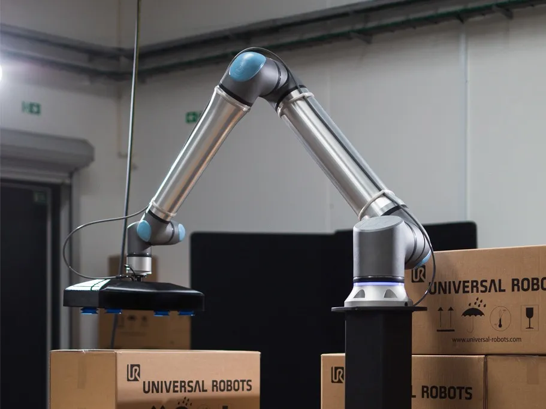
\includegraphics[width=0.60\textwidth]{images/UR20}
    \caption{UR20 Palletizing concept image}
\end{figure}